\documentclass[
11pt, % The default document font size, options: 10pt, 11pt, 12pt
%codirector, % Uncomment to add a codirector to the title page
]{charter} 

\usepackage{pgfgantt}



% El títulos de la memoria, se usa en la carátula y se puede usar el cualquier lugar del documento con el comando \ttitle
\titulo{Sistema de control y monitoreo de tiempo de abastecimiento de camiones basado en una OrangePI5} 

% Nombre del posgrado, se usa en la carátula y se puede usar el cualquier lugar del documento con el comando \degreename
\posgrado{Carrera de Especialización en Sistemas Embebidos} 
%\posgrado{Carrera de Especialización en Internet de las Cosas} 
%\posgrado{Carrera de Especialización en Intelegencia Artificial}
%\posgrado{Maestría en Sistemas Embebidos} 
%\posgrado{Maestría en Internet de las cosas}

% Tu nombre, se puede usar el cualquier lugar del documento con el comando \authorname
\autor{Anthony Martyn Maisincho Jivaja} 

% El nombre del director y co-director, se puede usar el cualquier lugar del documento con el comando \supname y \cosupname y \pertesupname y \pertecosupname
\director{MSc. Jefferson Cunalata}
\pertenenciaDirector{SIEMAV S.A} 
% FIXME:NO IMPLEMENTADO EL CODIRECTOR ni su pertenencia
\codirector{John Doe} % para que aparezca en la portada se debe descomentar la opción codirector en el documentclass
\pertenenciaCoDirector{FIUBA}

% Nombre del cliente, quien va a aprobar los resultados del proyecto, se puede usar con el comando \clientename y \empclientename
\cliente{MSc. Geovanny Arguello}
\empresaCliente{SIEMAV S.A}

% Nombre y pertenencia de los jurados, se pueden usar el cualquier lugar del documento con el comando \jurunoname, \jurdosname y \jurtresname y \perteunoname, \pertedosname y \pertetresname.
\juradoUno{Nombre y Apellido (1)}
\pertenenciaJurUno{pertenencia (1)} 
\juradoDos{Nombre y Apellido (2)}
\pertenenciaJurDos{pertenencia (2)}
\juradoTres{Nombre y Apellido (3)}
\pertenenciaJurTres{pertenencia (3)}
 
\fechaINICIO{22 de agosto de 2023}		%Fecha de inicio de la cursada de GdP \fechaInicioName
\fechaFINALPlan{10 de octubre de 2023} 	%Fecha de final de cursada de GdP
\fechaFINALTrabajo{15 de mayo de 2024}	%Fecha de defensa pública del trabajo final


\begin{document}

\maketitle
\thispagestyle{empty}
\pagebreak


\thispagestyle{empty}
{\setlength{\parskip}{0pt}
\tableofcontents{}
}
\pagebreak


\section*{Registros de cambios}
\label{sec:registro}


\begin{table}[ht]
\label{tab:registro}
\centering
\begin{tabularx}{\linewidth}{@{}|c|X|c|@{}}
\hline
\rowcolor[HTML]{C0C0C0} 
Revisión & \multicolumn{1}{c|}{\cellcolor[HTML]{C0C0C0}Detalles de los cambios realizados} & Fecha      \\ \hline
0      & Creación del documento                                 &\fechaInicioName \\ \hline
1.0    & Se completa hasta el punto 5                           & 07/09/2023 \\ \hline
2.0    & Se completa hasta el punto 9 y se hacen correciones    & 14/09/2023 \\ \hline
3.0    & Se completa hasta el punto 12 y se hacen correciones    & 26/09/2023 \\ \hline

%		  Se puede agregar algo más \newline
%		  En distintas líneas \newline
%		  Así                                                    & dd/mm/aaaa \\ \hline
%3      & Se completa hasta el punto 11 inclusive                & dd/mm/aaaa \\ \hline
%4      & Se completa el plan	                                 & dd/mm/aaaa \\ \hline
\end{tabularx}
\end{table}

\pagebreak



\section*{Acta de constitución del proyecto}
\label{sec:acta}

\begin{flushright}
Guayaquil, \fechaInicioName
\end{flushright}

\vspace{2cm}

Por medio de la presente se acuerda con el Ing. \authorname\hspace{1px} que su Trabajo Final de la \degreename\hspace{1px} se titulará ``\ttitle'', consistirá esencialmente en integrar en una OrangePI5 funcionalidades de un controlador lógico programable y ejecutar algoritmo de detección de objetos en videos en tiempo real, y tendrá un presupuesto preliminar estimado de 600 h de trabajo y \$10145 USD, con fecha de inicio \fechaInicioName\hspace{1px} y fecha de presentación pública \fechaFinalName.

Se adjunta a esta acta la planificación inicial.

\vfill

% Esta parte se construye sola con la información que hayan cargado en el preámbulo del documento y no debe modificarla
\begin{table}[ht]
\centering
\begin{tabular}{ccc}
\begin{tabular}[c]{@{}c@{}}Dr. Ing. Ariel Lutenberg \\ Director posgrado FIUBA\end{tabular} & \hspace{2cm} & \begin{tabular}[c]{@{}c@{}}\clientename \\ \empclientename \end{tabular} \vspace{2.5cm} \\ 
\multicolumn{3}{c}{\begin{tabular}[c]{@{}c@{}} \supname \\ Director del Trabajo Final\end{tabular}} \vspace{2.5cm} \\
%\begin{tabular}[c]{@{}c@{}}\jurunoname \\ Jurado del Trabajo Final\end{tabular}     &  & \begin{tabular}[c]{@{}c@{}}\jurdosname\\ Jurado del Trabajo Final\end{tabular}  \vspace{2.5cm}  \\
%\multicolumn{3}{c}{\begin{tabular}[c]{@{}c@{}} \jurtresname\\ Jurado del Trabajo Final\end{tabular}} \vspace{.5cm}                                                                     
\end{tabular}
\end{table}




\section{1. Descripción técnica-conceptual del proyecto a realizar}
\label{sec:descripcion}

SIEMAV S.A, se dedica a generar soluciones tecnológicas innovadoras mediante el desarrollo de hardware y software a medida con el objetivo de mejorar la competitividad de sus clientes y optimizar su productividad. Actualmente uno de sus clientes requiere mejorar los tiempos de abastecimiento de camiones en uno de sus centros de distribución. 

SIEMAV S.A propuso un sistema basado en un controlador lógico programable (PLC) y una mini CPU de altas prestaciones. El PLC, actualmente se encarga del control del tablero eléctrico, mientras que la CPU es empleada para ejecutar el algoritmo de detección de objetos en imágenes y videos en tiempo real.

Siempre buscando optimizar recursos y abaratar costos al producto final, se planteó utilizar un sistema embebido que sea capaz de asumir el rol del PLC y la CPU. Para esto se debe reestructurar el proyecto e integrar todo el sistema en una ORANGEPI5. Actualmente, este SBC (\textit{System board Computer}) no ha sido utilizado en la empresa. Por lo tanto, se tiene como desafío migrar toda la funcionalidad del sistema en una sola placa embebida. 

Utilizar una sola placa embebida como la ORANGEPI5 es una solución altamente eficiente y coste-efectiva. Al integrar todas las funcionalidades en este equipo se disminuirá la complejidad de la infraestructura. Además,  se aprovechará su unidad de procesamiento de redes neuronales para la detección de los camiones parqueados y también sus periféricos para el control del tablero. Esta integración permitirá  una mayor eficiencia energética, ahorro en términos de hardware, espacio físico, mantenimiento y optimización de recursos. 

En la Figura \ref{fig:diagBloques} se presenta el diagrama en bloques del sistema. Se identifican tres fases, la primera es el montaje del algoritmo YOLOV8. La segunda es la comunicación y el manejo de la placa PLC SIEMAV, que permitirá controlar el tablero eléctrico. Finalmente, comunicación con cámaras IP y tablero LED, importante para la obtención de datos de imágenes e interfaz visual para los operadores, respectivamente.
\begin{figure}[htpb]
\centering 
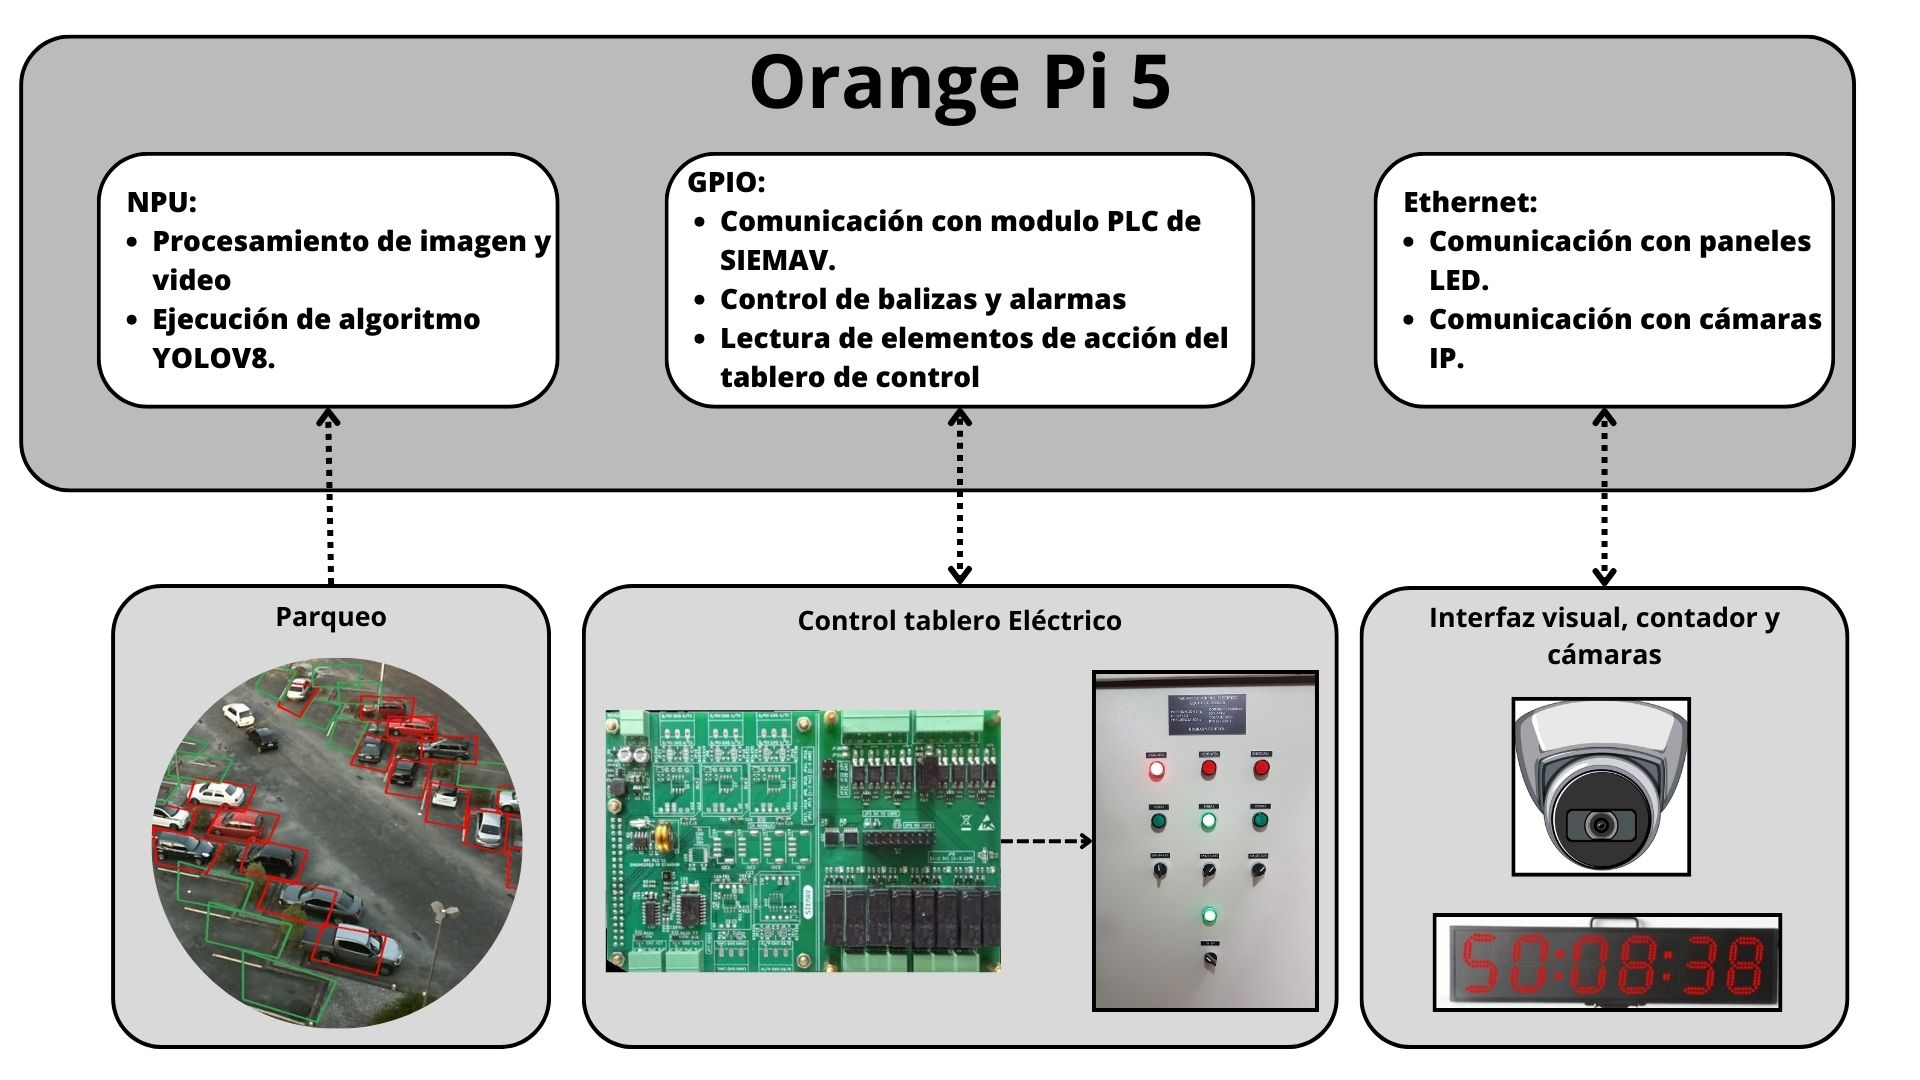
\includegraphics[width=1\textwidth]{./Figuras/diagramabloques.jpg}
\caption{Diagrama en bloques del sistema}
\label{fig:diagBloques}
\end{figure}

\vspace{25px}


\section{2. Identificación y análisis de los interesados}
\label{sec:interesados}

\begin{table}[ht]
%\caption{Identificación de los interesados}
%\label{tab:interesados}
\begin{tabularx}{\linewidth}{@{}|l|X|X|l|@{}}
\hline
\rowcolor[HTML]{C0C0C0} 
Rol           & Nombre y Apellido & Organización 	& Puesto 	\\ \hline
Auspiciante   & -                 &   SIEMAV S.A    &-         	\\ \hline
Cliente       & \clientename      &\empclientename	& C.T.O       	\\ \hline
Responsable   & \authorname       & FIUBA        	& Alumno 	\\ \hline
Colaboradores &Ing. Alexis Mora& SIEMAV S.A      & Consultor firmware\\ \hline
Orientador    & \supname	      & \pertesupname 	& Director Trabajo final \\ \hline
\end{tabularx}
\end{table}

\begin{itemize}
	\item Auspiciante: SIEMAV S.A que impulsa el desarrollo tecnológico, un gran apoyo en adquisición de todos los equipos necesarios.
	\item Equipo: Alexis Mora, jefe de investigación y desarrollo, experto en miniordenadores como la OrangePI5 y con buen criterio al momento de desarrollar proyectos.
	\item Orientador: con amplia trayectoria en el desarrollo de hardware y firmware para sistemas embebidos, ayudará mucho con soporte, consultoría y objetivos del proyecto.
\end{itemize}


\section{3. Propósito del proyecto}
\label{sec:proposito}
El propósito del proyecto es integrar todo el sistema de control y monitoreo de tiempo de abastecimiento de camiones en un solo sistema embebido. Con esto se quiere lograr un sistema más económico, reducir la complejidad de la infraestructura y aprovechar al máximo la OrangePI5.

\section{4. Alcance del proyecto}
\label{sec:alcance}
Las actividades dentro del alcance del proyecto consiste en lo siguiente:
\begin{itemize}
	\item Estudio de la tarjeta PLC de la empresa auspiciante.
	\item Adaptación y correciones del hardware actual de la tarjeta PLC para que funcione con la OrangePI5. 
	\item Desarrollo de software para manejo de la tarjeta PLC de SIEMAV y pruebas de su funcionamiento.
	\item Desarrollo de software para el manejo del tablero LED.
	\item Estudio de cómo usar la NPU de la OrangePI5.
	\item Integrar algoritmo de detección de objetos e imágenes YOLOV8 en la ORANGEPI5 usando la NPU.
	\item Estudio de como integrar diferentes tareas en una ORANGEPI5, ya que se debe interactuar con la tarjeta PLC, extraer imágenes y procesarlas y comunicarse con tableros LED.
\end{itemize}
Las actividades fuera del alcance del proyecto son las siguientes:
\begin{itemize}
	\item Entrenamiento del algoritmo de detección de imágenes.
	\item Correcciones a características de funcionamiento del algoritmo YOLOV8.
	\item Implementación del tablero de control eléctrico.
	\item Instalación en campo del sistema.
\end{itemize}

\section{5. Supuestos del proyecto}
\label{sec:supuestos}


Para el desarrollo del presente proyecto se supone que:

\begin{itemize}
	\item La importación de la ORANGEPI5 no tomará más de un mes.
	\item Correr el algoritmo de detección de objetos e imágenes en la OrangePI5 no implicará profundizar en este tema.
	\item Se dispondrá de todos los recursos necesarios como placa, cámaras, tablero LED para el desarrollo eficiente del proyecto.
	\item La versión actual de la tarjeta Módulo PLC de SIEMAV, no requerirá de extensas modificaciones para la adaptación a la OrangePI5.
	\item Tomará menos de tres meses disponer del nuevo "Módulo PLC".
	\item Habrá un seguimiento por parte del director y del colaborador del proyecto mensualmente.
\end{itemize}


\section{6. Requerimientos}
\label{sec:requerimientos}

\begin{enumerate}
	\item Requerimientos funcionales
		\begin{enumerate}
			\item El sistema debe reconocer cuando un camión de abastecimiento se encuentra parqueado.
			\item El sistema debe registrar el tiempo que se tomó durante el abastecimiento.
			\item El usuario debe poder visualizar el número de andén y el tiempo transcurrido durante el abastecimiento.
			\item El usuario reconocerá el estado del sistema visualizando las balizas.
			\item El sistema debe tener dos modos de funcionamiento, manual y automático.
			\item El usuario debe poder operar el sistema en modo manual mediante un tablero de control.
		\end{enumerate}
	\item Requerimientos del controlador del tablero eléctrico
		\begin{enumerate}
			\item La OrangePI5 debe leer estado de selectores, pulsadores, contactos auxiliares y paro de emergencia.
			\item La OrangePI5 controlará las balizas mediante el manejo de las salidas de la tarjeta PLC de SIEMAV.
			\item La OrangePI5 controlará las luces piloto verde y rojo mendiante la tarjeta PLC de SIEMAV.
			\item Dentro del tablero se tendrá la OrangePI5 como tarjeta maestro o controladora del sistema.
		\end{enumerate}
	\item Requerimiento de interfaz de usuario
		\begin{enumerate}
			\item El tablero, mediante sus luces piloto verde y rojo por andén, indicarán el estado de inicio y final del proceso.
			\item Un selector de tres posiciones por andén establecerá el modo de funcionamiento del tablero, cuando el selector esté a la izquierda estaremos en modo manual, en el caso de la derecha modo automático, y cuando se encuentre en el centro, signica que ese andén esta fuera de servicio.
			\item Se contará con dos pulsadores por andén, estos serán utilizados en el caso de que estemos en modo manual, cuando se presiona el pulsador uno significa que el parqueo o andén esta ocupado, cuando se presiona el pulsador dos, signica que el andén ha sido desocupado.
			\item Cuando estamos en modo manual y se utilizan los pulsadores, el sistema tendrá que iniciar la cuenta, mostrar en las balizas el estado del proceso e indicar el tiempo en el tablero LED.
			\item Cada andén tendrá una baliza, el color verde indica que hay tiempo y el rojo que se expiró el tiempo.
			\item Se utilizará tableros LED como cronómetros digitales, donde el usuario tendrá información del tiempo actual.
		\end{enumerate}
	\item Requerimientos de software
		\begin{enumerate}
			\item Cuando el tablero esté en modo automático, el software debe detectar cuando un andén es ocupado por el camión, mediante el algoritmo de detección de objetos, posterior a esto se inicia el temporizador.
			\item Cuando se detecte el camión en el andén, el software debe guardar la hora de entrada.
			\item Cuando el camión desocupe el andén, se  debe registrar la hora de salida.
			\item La creación de la API que controlará la tarjeta PLC de SIEMAV, será desarrollado en python.
			\item Se desarrollará una API en python para controlar los tableros de LED.
			\item Se debe utilizar la NPU de la OrangePI5 para el procesamiento de imágenes y vídeos.
		\end{enumerate}
	\item Requerimientos de diseño
		\begin{enumerate}
			\item El SBC a utilizar será la OrangePI5.
		\end{enumerate}
\end{enumerate}

\section{7. Historias de usuarios (\textit{Product backlog})}
\label{sec:backlog}
Las historias de usuario llevarán un puntaje según 3 aspectos:
\begin{itemize}
	\item Dificultad: cantidad de trabajo a realizar.
	\item Complejidad: nivel de sofisticación del trabajo.
	\item Incertidumbre: nivel de riesgo que involucra realizar la tarea.
\end{itemize}

\begin{enumerate}
	\item Como gerente tecnológico, deseo aprovechar al máximo la OrangePI5 para evitar tener que comprar un componente de hardware adicional.
		\begin{itemize}
			\item Dificultad: 3
			\item Complejidad: 5
			\item Incertidumbre: 5
			\item Total: 13
		\end{itemize}
	\item Como operador de abastecimiento, deseo tener información del tiempo transcurrido durante la maniobra, para cumplir con los tiempos de abastecimiento.
		\begin{itemize}
			\item Dificultad: 1
			\item Complejidad: 1
			\item Incertidumbre: 1
			\item Total: 3
		\end{itemize}	
	\item Como programador del PLC de SIEMAV, deseo tener una API práctica y sencilla, para manejar las entradas y salidas de la tarjeta.
		\begin{itemize}
			\item Dificultad: 5
			\item Complejidad: 3
			\item Incertidumbre: 1
			\item Total: 13 
		\end{itemize}	
	\item Como gerente tecnológico, deseo usar la NPU de la OrangePI5 para el procesamiento de imágenes y vídeos.
		\begin{itemize}
			\item Dificultad: 5
			\item Complejidad: 5
			\item Incertidumbre: 5
			\item Total: 21
		\end{itemize}
\end{enumerate}
\section{8. Entregables principales del proyecto}
\label{sec:entregables}


Los entregables del proyecto son:

\begin{itemize}
	\item Documentación de uso de la NPU en la OrangePI5
	\item Repositorio de Github con los códigos desarrollados para la Implementación de las API's
	\item Informe final
\end{itemize}



\section{9. Desglose del trabajo en tareas}
\label{sec:wbs}

\begin{enumerate}
\item Planificación y gestión del proyecto (115 hs)
	\begin{enumerate}
	\item Desarrollo del plan de trabajo (20 hs)
	\item Informe de avances (15 hs)
	\item Preparación de la memoria de trabajo (40 hs)
	\item Redacción de la memoria de trabajo (40 hs)
	\end{enumerate}
\item Investigación preliminar (100 hs)
	\begin{enumerate}
	\item Arquitectura y periféricos de la OrangePI5 (20 hs)
	\item Uso de la NPU en la OrangePI5 (20 hs)
	\item Estudio de protocolo UDP (20 hs)
	\item Algoritmo YOLOV8 y su aplicación usando python (40 hs)
	\end{enumerate}
\item Desarrollo de firmware (65 hs)
	\begin{enumerate}
	\item Preparación del framework (5 hs)
	\item Módulo para manejo de tarjeta PLC de SIEMAV (20 hs)
	\item Creación de API para control de PLC de SIEMAV (10 hs)
	\item Módulo para control de tablero de LED basado en tramas UDP (20 hs)
	\item API para trama UDP (10 hs)
	\end{enumerate}
\item Uso de la NPU (100 hs)
	\begin{enumerate}
	\item Adaptación del algoritmo YOLOV8 a la OrangePI5 (40 hs)
	\item Testeo del algoritmo utilizando la NPU (20 hs)
	\item Pruebas de rendimiento  (20 hs)
	\item Ajustes y corrección de errores (20 hs)
	\end{enumerate}
\item Inplementación del software de la aplicación (130 hs)
	\begin{enumerate}
	\item Importación de bibliotecas y módulos creados (10 hs)
	\item Diseño conceptual de la aplicación (20 hs)
	\item Adaptación de las diferentes tareas a la aplicación  (40 hs)
	\item Operación manual de la aplicación (20 hs)
	\item Operación automática de la aplicación (20 hs)
	\item Testeo de la aplicación (20 hs)
	\end{enumerate}
\item Pruebas finales (120 hs)
	\begin{enumerate}
	\item Prueba del modo manual (20 hs)
	\item Prueba del modo automático (20 hs)
	\item Rendimiento de la OrangePI5 durante todo el proceso (40 hs)
	\item Depuración y corrección de errores (20 hs)
	\end{enumerate}
\end{enumerate}

Cantidad total de horas: (630 hs)





\section{10. Diagrama de Activity On Node}
\label{sec:AoN}

Se muestra en la Figura \ref{fig:AoN} el diagrama \textit{Activity on Node}, donde la variable \textit{t} representa las horas que tomará la tarea. El camino crítico marcado en negrita indica que el proyecto puede finalizarse en un tiempo mínimo de 565 horas.


\begin{figure}[htpb]
\centering 
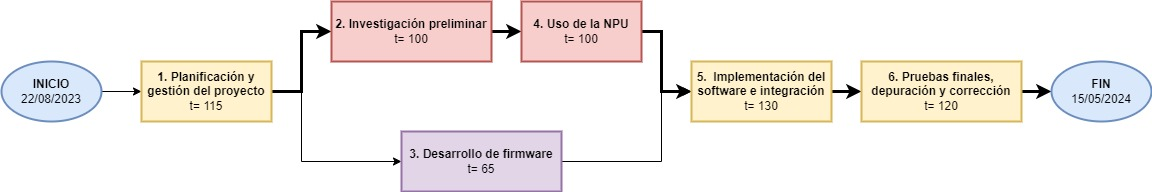
\includegraphics[width=1.1\textwidth]{./Figuras/Activity on node.jpg}
\caption{Diagrama de \textit{Activity on Node}.}
\label{fig:AoN}
\end{figure}



\section{11. Diagrama de Gantt}
\label{sec:gantt}

El siguiente \textit{Diagrama de Gantt} fue elaborado en base a una carga semanal de veinte horas, donde se incluyen los sábados y domingos como días laborables.

\begin{landscape}
\begin{ganttchart}[
	hgrid,
	vgrid,
	x unit=0.07cm,
	y unit chart=0.65cm,
	time slot format=isodate,
	time slot unit=day,
	bar/.append style={fill=green!30},
	group/.append style={fill=green!50},
	link/.style={->, thick}
	]{2023-08-23}{2024-05-15}
	
	\gantttitlecalendar{year, month} \\
	
	\ganttgroup{1 Gestión del proyecto}{2023-08-23}{2024-05-05} \\
	\ganttbar{1.1 Plan de trabajo}{2023-08-23}{2023-08-28} \\
	\ganttbar{1.2 Memoria de trabajo}{2024-04-15}{2024-05-05} \\
	
	\ganttgroup{2 Investigación}{2023-10-16}{2023-11-19} \\
	\ganttbar{2.1 Arquitectura y periféricos OPI5}{2023-10-16}{2023-10-22} \\
	\ganttbar{2.2 NPU de la OPI5}{2023-10-23}{2023-10-29} \\
	\ganttbar{2.3 Protocolo UDP}{2023-10-30}{2023-11-05} \\
	\ganttbar{2.3 Algoritmo YOLOV8}{2023-11-06}{2023-11-19} \\
	
	\ganttgroup{3 Firmware}{2023-11-20}{2023-12-15} \\
	\ganttbar{3.1 Preparación framework}{2023-11-20}{2023-11-22} \\
	\ganttbar{3.2 Módulo tarjeta PLC SIEMAV}{2023-11-23}{2023-11-30} \\
	\ganttbar{3.3 API para tarjeta PLC SIEMAV}{2023-12-01}{2023-12-03} \\
	\ganttbar{3.4 Módulo para tablero LED}{2023-12-04}{2023-12-10} \\
	\ganttbar{3.4 API para tablero LED}{2023-12-11}{2023-12-15} \\

	\ganttgroup{4 Uso de la NPU}{2023-12-16}{2024-01-24} \\
	\ganttbar{4.1 YOLOV8 en la OPI5}{2023-12-16}{2023-12-30} \\
	\ganttbar{4.2 Test algoritmo YOLOV8}{2024-01-03}{2024-01-10} \\
	\ganttbar{4.3 Pruebas de rendimiento}{2024-01-11}{2024-01-17} \\
	\ganttbar{4.4 Ajustes y corrección de errores}{2024-01-18}{2024-01-24} \\
	
\end{ganttchart}
\end{landscape}

\begin{landscape}
	\begin{ganttchart}[
		hgrid,
		vgrid,
		x unit=0.07cm,
		y unit chart=0.65cm,
		time slot format=isodate,
		time slot unit=day,
		bar/.append style={fill=green!30},
		group/.append style={fill=green!50},
		link/.style={->, thick}
		]{2023-08-23}{2024-05-15}
		
		\gantttitlecalendar{year, month} \\
		
		\ganttgroup{5 Integración software}{2024-01-25}{2024-03-10} \\
		\ganttbar{5.1 Uso de módulos y bibliotecas}{2024-01-25}{2024-01-28} \\
		\ganttbar{5.2 Diseño conceptual de la aplicación}{2024-01-29}{2024-02-04} \\
		\ganttbar{5.3 Adaptación y gestión de procesos}{2024-02-05}{2024-02-18} \\
		\ganttbar{5.4 Modo manual}{2024-02-19}{2024-02-25} \\
		\ganttbar{5.5 Modo automático}{2024-02-26}{2024-03-03} \\
		\ganttbar{5.6 Testeo de la aplicación}{2024-03-04}{2024-03-10} \\
		
		\ganttgroup{6 Pruebas finales}{2024-03-11}{2023-12-15} \\
		\ganttbar{6.1 Test modo manual}{2024-03-11}{2024-03-17} \\
		\ganttbar{6.2 Test modo auto}{2024-03-18}{2024-03-24} \\
		\ganttbar{6.3 Pruebas de rendimiento OPI5}{2024-03-25}{2024-04-07} \\
		\ganttbar{6.4 Depuración y correción de errores}{2024-04-08}{2024-04-14} \\
		
	\end{ganttchart}
	\end{landscape}
	
	


\section{12. Presupuesto detallado del proyecto}
\label{sec:presupuesto}

\begin{table}[htpb]
	\centering
	\caption{Costos del proyecto de tesis.}
	\label{tab:presupuesto}
	\small
	\begin{tabularx}{\linewidth}{@{}|X|c|r|r|@{}}
	\hline
	\rowcolor[HTML]{C0C0C0} 
	\multicolumn{4}{|c|}{\cellcolor[HTML]{C0C0C0}COSTOS DIRECTOS} \\ \hline
	\rowcolor[HTML]{C0C0C0} 
	 &
	  \multicolumn{1}{c|}{\cellcolor[HTML]{C0C0C0}Cantidad} &
	  \multicolumn{1}{c|}{\cellcolor[HTML]{C0C0C0}Valor unitario} &
	  \multicolumn{1}{c|}{\cellcolor[HTML]{C0C0C0}Valor total} \\ 
	\rowcolor[HTML]{C0C0C0} Descripción  &
	  \multicolumn{1}{c|}{\cellcolor[HTML]{C0C0C0}} &
	  \multicolumn{1}{c|}{\cellcolor[HTML]{C0C0C0} \$ USD} &
	  \multicolumn{1}{c|}{\cellcolor[HTML]{C0C0C0} \$ USD} \\ \hline
	  
	\multicolumn{4}{|c|}{\textbf{MATERIALES Y SUMINISTROS}}\\ \hline
	OrangePI5 	& \multicolumn{1}{c|}{	1	} & \multicolumn{1}{c|}{	200	} &  \multicolumn{1}{c|}{	200	} \\ \hline
	Tarjeta controladora esclavo	& \multicolumn{1}{c|}{	2	} & \multicolumn{1}{c|}{	320	} &  \multicolumn{1}{c|}{	640	} \\ \hline
	Tarjeta controladora maestro		& \multicolumn{1}{c|}{	1	} & \multicolumn{1}{c|}{	560	} &  \multicolumn{1}{c|}{	560	} \\ \hline
	Cámaras	IP + Algoritmo machine learning		& \multicolumn{1}{c|}{	1	} & \multicolumn{1}{c|}{	550	} &  \multicolumn{1}{c|}{	550	} \\ \hline
	Tablero LED para exteriores			& \multicolumn{1}{c|}{	1	} & \multicolumn{1}{c|}{	650	} &  \multicolumn{1}{c|}{	650	} \\ \hline
	Memoria SD			& \multicolumn{1}{c|}{	1	} & \multicolumn{1}{c|}{	20	} &  \multicolumn{1}{c|}{	20	} \\ \hline
	Batería					& \multicolumn{1}{c|}{	4	} & \multicolumn{1}{c|}{	10	} &  \multicolumn{1}{c|}{	40	} \\ \hline

	
	\multicolumn{4}{|c|}{\textbf{OTROS COSTOS DIRECTOS}}\\ \hline
	Imprevistos	($\sim$10\% del total del  proyecto)				& \multicolumn{1}{c|}{	1	} & \multicolumn{1}{c|}{	266	} &  \multicolumn{1}{c|}{	266	} \\ \hline
	
	\multicolumn{3}{|c|}{SUBTOTAL COSTOS DIRECTOS} & \multicolumn{1}{c|}{ 2.926 } \\ \hline
	
	\rowcolor[HTML]{C0C0C0} 
	\multicolumn{4}{|c|}{\cellcolor[HTML]{C0C0C0}COSTOS INDIRECTOS} \\ \hline
	\rowcolor[HTML]{C0C0C0} 
	 &
	  \multicolumn{1}{c|}{\cellcolor[HTML]{C0C0C0}Cantidad} &
	  \multicolumn{1}{c|}{\cellcolor[HTML]{C0C0C0}Valor unitario} &
	  \multicolumn{1}{c|}{\cellcolor[HTML]{C0C0C0}Valor total} \\  
	\rowcolor[HTML]{C0C0C0} Descripción  &
	\multicolumn{1}{c|}{\cellcolor[HTML]{C0C0C0}} &
	\multicolumn{1}{c|}{\cellcolor[HTML]{C0C0C0} \$ USD} &
	\multicolumn{1}{c|}{\cellcolor[HTML]{C0C0C0} \$ USD} \\ \hline
	Alquiler, mantenimiento y servicios generales del lugar de trabajo	& \multicolumn{1}{c|}{	8	} & \multicolumn{1}{c|}{	100	} &  \multicolumn{1}{c|}{	800	} \\ \hline
	
	\multicolumn{3}{|c|}{SUBTOTAL COSTOS INDIRECTOS} &
	  \multicolumn{1}{c|}{800 } \\ \hline
	\rowcolor[HTML]{C0C0C0}
	\multicolumn{3}{|c|}{TOTAL} &
	\multicolumn{1}{c|}{ 3.726 }
	   \\ \hline
	\end{tabularx}%
	\end{table}

\section{13. Gestión de riesgos}
\label{sec:riesgos}

\begin{consigna}{red}
a) Identificación de los riesgos (al menos cinco) y estimación de sus consecuencias:
 
Riesgo 1: detallar el riesgo (riesgo es algo que si ocurre altera los planes previstos de forma negativa)
\begin{itemize}
	\item Severidad (S): mientras más severo, más alto es el número (usar números del 1 al 10).\\
	Justificar el motivo por el cual se asigna determinado número de severidad (S).
	\item Probabilidad de ocurrencia (O): mientras más probable, más alto es el número (usar del 1 al 10).\\
	Justificar el motivo por el cual se asigna determinado número de (O). 
\end{itemize}   

Riesgo 2:
\begin{itemize}
	\item Severidad (S): 
	\item Ocurrencia (O):
\end{itemize}

Riesgo 3:
\begin{itemize}
	\item Severidad (S): 
	\item Ocurrencia (O):
\end{itemize}


b) Tabla de gestión de riesgos:      (El RPN se calcula como RPN=SxO)

\begin{table}[htpb]
\centering
\begin{tabularx}{\linewidth}{@{}|X|c|c|c|c|c|c|@{}}
\hline
\rowcolor[HTML]{C0C0C0} 
Riesgo & S & O & RPN & S* & O* & RPN* \\ \hline
       &   &   &     &    &    &      \\ \hline
       &   &   &     &    &    &      \\ \hline
       &   &   &     &    &    &      \\ \hline
       &   &   &     &    &    &      \\ \hline
       &   &   &     &    &    &      \\ \hline
\end{tabularx}%
\end{table}

Criterio adoptado: 
Se tomarán medidas de mitigación en los riesgos cuyos números de RPN sean mayores a...

Nota: los valores marcados con (*) en la tabla corresponden luego de haber aplicado la mitigación.

c) Plan de mitigación de los riesgos que originalmente excedían el RPN máximo establecido:
 
Riesgo 1: plan de mitigación (si por el RPN fuera necesario elaborar un plan de mitigación).
  Nueva asignación de S y O, con su respectiva justificación:
  - Severidad (S): mientras más severo, más alto es el número (usar números del 1 al 10).
          Justificar el motivo por el cual se asigna determinado número de severidad (S).
  - Probabilidad de ocurrencia (O): mientras más probable, más alto es el número (usar del 1 al 10).
          Justificar el motivo por el cual se asigna determinado número de (O).

Riesgo 2: plan de mitigación (si por el RPN fuera necesario elaborar un plan de mitigación).
 
Riesgo 3: plan de mitigación (si por el RPN fuera necesario elaborar un plan de mitigación).

\end{consigna}


\section{14. Gestión de la calidad}
\label{sec:calidad}

\begin{consigna}{red}
Elija al menos diez requerientos que a su criterio sean los más importantes/críticos/que aportan más valor y para cada uno de ellos indique las acciones de verificación y validación que permitan asegurar su cumplimiento.

\begin{itemize} 
\item Req \#1: copiar acá el requerimiento.

\begin{itemize}
	\item Verificación para confirmar si se cumplió con lo requerido antes de mostrar el sistema al cliente. Detallar 
	\item Validación con el cliente para confirmar que está de acuerdo en que se cumplió con lo requerido. Detallar  
\end{itemize}

\end{itemize}

Tener en cuenta que en este contexto se pueden mencionar simulaciones, cálculos, revisión de hojas de datos, consulta con expertos, mediciones, etc.  Las acciones de verificación suelen considerar al entregable como ``caja blanca'', es decir se conoce en profundidad su funcionamiento interno.  En cambio, las acciones de validación suelen considerar al entregable como ``caja negra'', es decir, que no se conocen los detalles de su funcionamiento interno.

\end{consigna}

\section{15. Procesos de cierre}    
\label{sec:cierre}

\begin{consigna}{red}
Establecer las pautas de trabajo para realizar una reunión final de evaluación del proyecto, tal que contemple las siguientes actividades:

\begin{itemize}
	\item Pautas de trabajo que se seguirán para analizar si se respetó el Plan de Proyecto original:
	 - Indicar quién se ocupará de hacer esto y cuál será el procedimiento a aplicar. 
	\item Identificación de las técnicas y procedimientos útiles e inútiles que se emplearon, y los problemas que surgieron y cómo se solucionaron:
	 - Indicar quién se ocupará de hacer esto y cuál será el procedimiento para dejar registro.
	\item Indicar quién organizará el acto de agradecimiento a todos los interesados, y en especial al equipo de trabajo y colaboradores:
	  - Indicar esto y quién financiará los gastos correspondientes.
\end{itemize}

\end{consigna}


\end{document}
